\documentclass[border=15pt, multi, tikz]{standalone}
%\usepackage{blocks}
\usepackage{import}
\subimport{../layers/}{init}
\usetikzlibrary{positioning}
\usetikzlibrary{3d} %for including external image
\usepackage[utf8]{inputenc}
\def\ConvColor{rgb:yellow,5;red,7.5;white,5}
\def\ConvTColor{rgb:yellow,4;red,3;white,1}
\def\gConvTColor{rgb:yellow,8;red,3;white,1;green,4}
\def\eConvTColor{rgb:blue,8;red,3;white,4;green,6}
\def\eeConvTColor{rgb:red,10;blue,1;black,4;yellow,2}
\def\ConvReluColor{rgb:yellow,5;red,5;white,5}
\def\PoolColor{rgb:red,1;black,0.3}
\def\imageColor{rgb:white,10}
\def\bnColor{rgb:blue,5;white,3;green,2}
\def\lrColor{rgb:red,1;blue,1;white,3;black,2}
\def\FcColor{rgb:blue,8;red,2.5;white,5}
\def\FcReluColor{rgb:blue,5;red,5;white,4}
\def\SoftmaxColor{rgb:magenta,5;black,7}
\def\strideColor{rgb:black,5;white,3}
\newcommand{\up}{0.25}
\newcommand{\down}{0.25}
\newcommand{\arrowlength}{4}
\newcommand{\copymidarrow}{\tikz \draw[-Stealth,line width =0.8mm,draw={rgb:blue,4;red,1;green,1;black,3}] (-0.3,0) -- ++(0.3,0);}
\begin{document}
\begin{tikzpicture}
\tikzstyle{connection}=[ultra thick,every node/.style={sloped,allow upside
down},draw=\edgecolor,opacity=0.7]
\tikzstyle{copyconnection}=[ultra thick,every node/.style={sloped,allow upside down},draw={rgb:blue,1;red,10;green,1;black,3},opacity=0.7]
%%%%%%%%%%%%%%%%%%%%%%%%%%%%%%%%%%%%%%%%%%%%%%%%%%%%%%%%%%%%%%%%%%%%%%%%%%%%%%%%%%%%%%%%
%% Generator
%%%%%%%%%%%%%%%%%%%%%%%%%%%%%%%%%%%%%%%%%%%%%%%%%%%%%%%%%%%%%%%%%%%%%%%%%%%%%%%%%%%%%%%%
% Fully connected 1
\pic[shift={(0,0,0)}] at (0,0,0)
{Box={name=gfc1,caption=fc1,xlabel={"x"},zlabel=,fill=\FcColor,height=3,width=3,depth=100}};
% input image
\pic[shift={(0,-15,0)}] at (gfc1-south)
{Box={name=img_input,caption=input
image,xlabel={{"","dummy"}},ylabel=28,zlabel=28,opacity=1.0,fill=\imageColor,height=50,width=1,depth=50}};
\node[canvas is zy plane at x=0,shift={(0,0,0)}] (temp) at (img_input-east) {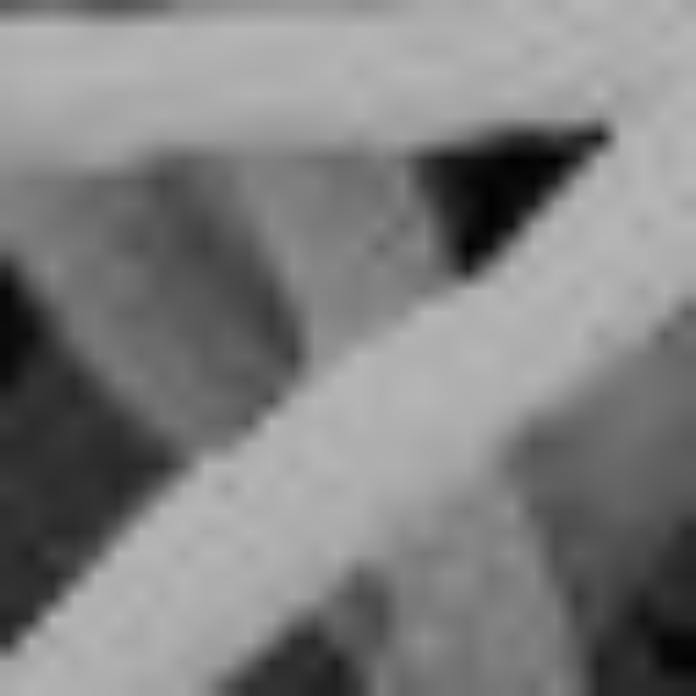
\includegraphics[width=10cm,height=10cm]{sencebgan_input}};

\pic[shift={(0,0,0)}] at (gfc1-east)
{RightBandedBox={name=gbnlr1,caption=bn1,zlabel=8192,fill=\bnColor,bandfill=\lrColor,height=3,
width=3,depth=100}};
% % conv1_1,bn_1, leakyrelu 1
% Stride of convolution
\pic[shift={(2,0,0)}] at (gbnlr1-east)
{Box={name=test,caption=Stride2,zlabel=5,ylabel=5,fill=\strideColor,height=5,
width=18,depth=5}};
\pic[shift={(2,0,0)}] at (gbnlr1-east)
{Box={name=gcvt1,caption=convt1,xlabel={{"512","dummy"}},ylabel=,zlabel=,fill=\gConvTColor,height=20,width=16,depth=20}};
\pic[shift={(0,0,0)}] at (gcvt1-east)
{RightBandedBox={name=gbnlr2,caption=,ylabel=2,zlabel=2,fill=\bnColor,bandfill=\lrColor,height=20,width=2,depth=20}};

% % conv1_1,bn_1, leakyrelu 1
% Stride of convolution
\pic[shift={(2,0,0)}] at (gbnlr2-east)
{Box={name=test,caption=Stride2,zlabel=5,ylabel=5,fill=\strideColor,height=5,
width=10,depth=5}};
\pic[shift={(2,0,0)}] at (gbnlr2-east)
{Box={name=gcvt2,caption=convt2,xlabel={{"256","dummy"}},ylabel=,zlabel=,fill=\gConvTColor,height=30,width=8,depth=30}};
\pic[shift={(0,0,0)}] at (gcvt2-east)
{RightBandedBox={name=gbnlr3,caption=,ylabel=7,zlabel=7,fill=\bnColor,bandfill=\lrColor,height=30,width=2,depth=30}};

% % conv1_1,bn_1, leakyrelu 1
% Stride of convolution
\pic[shift={(2,0,0)}] at (gbnlr3-east)
{Box={name=test,caption=Stride2,zlabel=5,ylabel=5,fill=\strideColor,height=5,
width=6,depth=5}};
\pic[shift={(2,0,0)}] at (gbnlr3-east)
{Box={name=gcvt3,caption=convt3,xlabel={{"128","dummy"}},ylabel=,zlabel=,fill=\gConvTColor,height=40,width=4,depth=40}};
\pic[shift={(0,0,0)}] at (gcvt3-east)
{RightBandedBox={name=gbnlr4,caption=,ylabel=14,zlabel=14,fill=\bnColor,bandfill=\lrColor,height=40,width=2,depth=40}};

% Final convolution
\pic[shift={(2,0,0)}] at (gbnlr4-east)
{Box={name=gcvt3,caption=convt4,xlabel={{"1","dummy"}},ylabel=28,zlabel=28,fill=\gConvTColor,height=50,width=2,depth=50}};


% Generated image
\pic[shift={(1,0,0)}] at (gcvt3-east)
{Box={name=img_gen,caption=generated
image,xlabel={{"","dummy"}},ylabel=28,zlabel=28,opacity=1.0,fill=\imageColor,height=50,width=1,depth=50}};
\node[canvas is zy plane at x=0,shift={(0,0,0)}] (temp) at (img_gen-east) {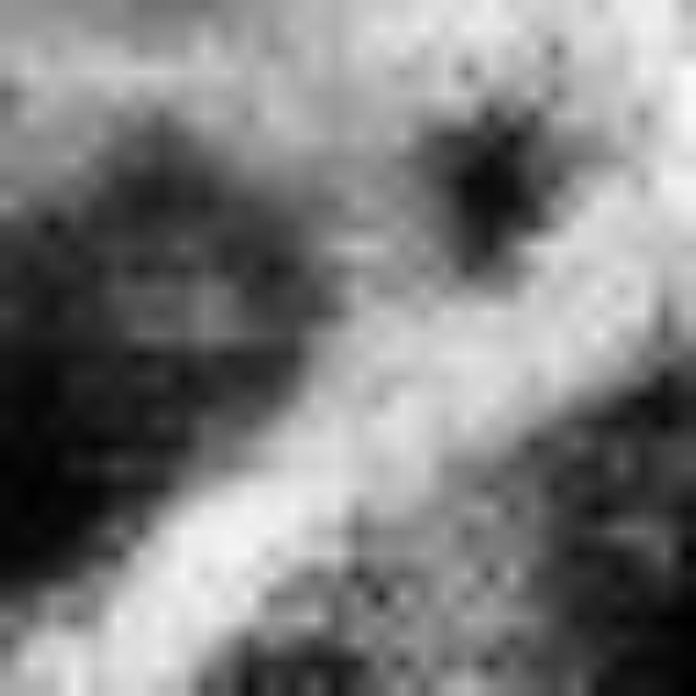
\includegraphics[width=10cm,height=10cm]{sencebgan_reconstruct}};
%%%%%%%%%%%%%%%%%%%%%%%%%%%%%%%%%%%%%%%%%%%%%%%%%%%%%%%%%%%%%%%%%%%%%%%%%%%%%%%%%%%%%%%%
%% Autoencoder
%%%%%%%%%%%%%%%%%%%%%%%%%%%%%%%%%%%%%%%%%%%%%%%%%%%%%%%%%%%%%%%%%%%%%%%%%%%%%%%%%%%%%%%%

%%%%%%%%%%%%%%%%%%%%%%%%%%%%%%%%%%%%%%%%%%%%%%%%%%%%%%%%%%%%%%%%%%%%%%%%%%%%%%%%%%%%%%%%
%% Encoder
%%%%%%%%%%%%%%%%%%%%%%%%%%%%%%%%%%%%%%%%%%%%%%%%%%%%%%%%%%%%%%%%%%%%%%%%%%%%%%%%%%%%%%%%
\pic[shift={(10 ,0,0)}] at (img_gen-east)
{Box={name=input_ae,caption=image,xlabel={{"","dummy"}},ylabel=32,zlabel=32,opacity=1.0,fill=\imageColor,height=50,width=1,depth=50}};
% % conv1_1,bn_1, leakyrelu 1
% Stride of convolution
\pic[shift={(2,0,0)}] at (input_ae-east)
{Box={name=test,caption=Stride2,zlabel=5,ylabel=5,fill=\strideColor,height=5,
width=2,depth=5}};
\pic[shift={(2,0,0)}] at (input_ae-east)
{Box={name=cvt1,caption=convt1,xlabel={{"128","dummy"}},ylabel=,zlabel=,fill=\ConvTColor,height=50,width=2,depth=50}};
\pic[shift={(0,0,0)}] at (cvt1-east)
{RightBandedBox={name=bnlr2,caption=,ylabel=16,zlabel=16,fill=\bnColor,bandfill=\lrColor,height=50,width=2,depth=50}};

% % conv1_1,bn_1, leakyrelu 1
% Stride of convolution
\pic[shift={(2,0,0)}] at (bnlr2-east)
{Box={name=test,caption=Stride2,zlabel=5,ylabel=5,fill=\strideColor,height=5,
width=4,depth=5}};
\pic[shift={(2,0,0)}] at (bnlr2-east)
{Box={name=cvt2,caption=convt2,xlabel={{"256","dummy"}},ylabel=,zlabel=,fill=\ConvTColor,height=40,width=4,depth=40}};
\pic[shift={(0,0,0)}] at (cvt2-east)
{RightBandedBox={name=bnlr3,caption=,ylabel=8,zlabel=8,fill=\bnColor,bandfill=\lrColor,height=40,width=2,depth=40}};

% % conv1_1,bn_1, leakyrelu 1
% Stride of convolution
\pic[shift={(2,0,0)}] at (bnlr3-east)
{Box={name=test,caption=Stride2,zlabel=5,ylabel=5,fill=\strideColor,height=5,
width=8,depth=5}};
\pic[shift={(2,0,0)}] at (bnlr3-east)
{Box={name=cvt3,caption=convt3,xlabel={{"512","dummy"}},ylabel=,zlabel=,fill=\ConvTColor,height=30,width=8,depth=30}};
\pic[shift={(0,0,0)}] at (cvt3-east)
{RightBandedBox={name=bnlr4,caption=,ylabel=4,zlabel=4,fill=\bnColor,bandfill=\lrColor,height=30,width=2,depth=30}};

% Final convolution
\pic[shift={(2,0,0)}] at (bnlr4-east)
{Box={name=cvt3,caption=latent representation,xlabel={{"1","dummy"}},ylabel=32,zlabel=32,fill=\ConvTColor,height=10,width=16,depth=10}};

%%%%%%%%%%%%%%%%%%%%%%%%%%%%%%%%%%%%%%%%%%%%%%%%%%%%%%%%%%%%%%%%%%%%%%%%%%%%%%%%%%%%%%%%
%% Decoder
%%%%%%%%%%%%%%%%%%%%%%%%%%%%%%%%%%%%%%%%%%%%%%%%%%%%%%%%%%%%%%%%%%%%%%%%%%%%%%%%%%%%%%%%
\pic[shift={(2,0,0)}] at (cvt3-east)
{Box={name=cv1,caption=conv1,xlabel={{"512","dummy"}},ylabel=,zlabel=,fill=\ConvColor,height=30,width=8,depth=30}};
\pic[shift={(0,0,0)}] at (cv1-east)
{RightBandedBox={name=bnlr_d1,caption=,ylabel=2,zlabel=2,fill=\bnColor,bandfill=\lrColor,height=30,width=2,depth=30}};

\pic[shift={(2,0,0)}] at (bnlr_d1-east)
{Box={name=cv2,caption=conv2,xlabel={{"256","dummy"}},ylabel=,zlabel=,fill=\ConvColor,height=35,width=4,depth=35}};
\pic[shift={(0,0,0)}] at (cv2-east)
{RightBandedBox={name=bnlr_d2,caption=,ylabel=4,zlabel=4,fill=\bnColor,bandfill=\lrColor,height=35,width=2,depth=35}};

\pic[shift={(2,0,0)}] at (bnlr_d2-east)
{Box={name=cv3,caption=conv3,xlabel={{"128","dummy"}},ylabel=,zlabel=,fill=\ConvColor,height=40,width=2,depth=40}};
\pic[shift={(0,0,0)}] at (cv3-east)
{RightBandedBox={name=bnlr_d3,caption=,ylabel=8,zlabel=8,fill=\bnColor,bandfill=\lrColor,height=40,width=2,depth=40}};

\pic[shift={(2,0,0)}] at (bnlr_d3-east)
{Box={name=cv4,caption=conv3,xlabel={{"64","dummy"}},ylabel=,zlabel=,fill=\ConvColor,height=45,width=2,depth=45}};
\pic[shift={(0,0,0)}] at (cv4-east)
{RightBandedBox={name=bnlr_d4,caption=,ylabel=16,zlabel=16,fill=\bnColor,bandfill=\lrColor,height=45,width=2,depth=45}};

\pic[shift={(2,0,0)}] at (bnlr_d4-east)
{Box={name=cv5,caption=conv3,xlabel={{"1","dummy"}},ylabel=,zlabel=,fill=\ConvColor,height=50,width=2,depth=50}};
\pic[shift={(0,0,0)}] at (cv5-east)
{RightBandedBox={name=bnlr_d5,caption=,ylabel=32,zlabel=32,fill=\bnColor,bandfill=\lrColor,height=50,width=2,depth=50}};

\pic[shift={(2,0,0)}] at (bnlr_d5-east)
{Box={name=output,caption=image',xlabel={{"","dummy"}},ylabel=32,zlabel=32,opacity=1.0,fill=\imageColor,height=50,width=1,depth=50}};

%%%%%%%%%%%%%%%%%%%%%%%%%%%%%%%%%%%%%%%%%%%%%%%%%%%%%%%%%%%%%%%%%%%%%%%%%%%%%%%%%%%%%%%%
%% Second Encoder
%%%%%%%%%%%%%%%%%%%%%%%%%%%%%%%%%%%%%%%%%%%%%%%%%%%%%%%%%%%%%%%%%%%%%%%%%%%%%%%%%%%%%%%%
% % conv1_1,bn_1, leakyrelu 1
% Stride of convolution
\pic[shift={(6,0,0)}] at (img_input-east)
{Box={name=etest,caption=Stride2,zlabel=5,ylabel=5,fill=\strideColor,height=5,
width=2,depth=5}};
\pic[shift={(6,0,0)}] at (img_input-east)
{Box={name=ecvt1,caption=convt1,xlabel={{"128","dummy"}},ylabel=,zlabel=,fill=\eConvTColor,height=50,width=2,depth=50}};
\pic[shift={(0,0,0)}] at (ecvt1-east)
{RightBandedBox={name=ebnlr2,caption=,ylabel=16,zlabel=16,fill=\bnColor,bandfill=\lrColor,height=50,width=2,depth=50}};

% % conv1_1,bn_1, leakyrelu 1
% Stride of convolution
\pic[shift={(2,0,0)}] at (ebnlr2-east)
{Box={name=etest,caption=Stride2,zlabel=5,ylabel=5,fill=\strideColor,height=5,
width=4,depth=5}};
\pic[shift={(2,0,0)}] at (ebnlr2-east)
{Box={name=ecvt2,caption=convt2,xlabel={{"256","dummy"}},ylabel=,zlabel=,fill=\eConvTColor,height=40,width=4,depth=40}};
\pic[shift={(0,0,0)}] at (ecvt2-east)
{RightBandedBox={name=ebnlr3,caption=,ylabel=8,zlabel=8,fill=\bnColor,bandfill=\lrColor,height=40,width=2,depth=40}};

% % conv1_1,bn_1, leakyrelu 1
% Stride of convolution
\pic[shift={(2,0,0)}] at (ebnlr3-east)
{Box={name=etest,caption=Stride2,zlabel=5,ylabel=5,fill=\strideColor,height=5,
width=8,depth=5}};
\pic[shift={(2,0,0)}] at (ebnlr3-east)
{Box={name=ecvt3,caption=convt3,xlabel={{"512","dummy"}},ylabel=,zlabel=,fill=\eConvTColor,height=30,width=8,depth=30}};
\pic[shift={(0,0,0)}] at (ecvt3-east)
{RightBandedBox={name=ebnlr4,caption=,ylabel=4,zlabel=4,fill=\bnColor,bandfill=\lrColor,height=30,width=2,depth=30}};

\pic[shift={(2,0,0)}] at (ebnlr4-east)
{Box={name=ecvt3,caption=latent representation,xlabel={{"1","dummy"}},ylabel=32,zlabel=32,fill=\eConvTColor,height=10,width=16,depth=10}};
%%%%%%%%%%%%%%%%%%%%%%%%%%%%%%%%%%%%%%%%%%%%%%%%%%%%%%%%%%%%%%%%%%%%%%%%%%%%%%%%%%%%%%%%
%% Third Encoder
%%%%%%%%%%%%%%%%%%%%%%%%%%%%%%%%%%%%%%%%%%%%%%%%%%%%%%%%%%%%%%%%%%%%%%%%%%%%%%%%%%%%%%%%
% % conv1_1,bn_1, leakyrelu 1
% Stride of convolution
\pic[shift={(5 ,-10,0)}] at (input_ae-south)
{Box={name=input_e3,caption=image,xlabel={{"","dummy"}},ylabel=32,zlabel=32,opacity=1.0,fill=\imageColor,height=50,width=1,depth=50}};
\node[canvas is zy plane at x=0,shift={(0,0,0)}] (temp) at (input_e3-east) {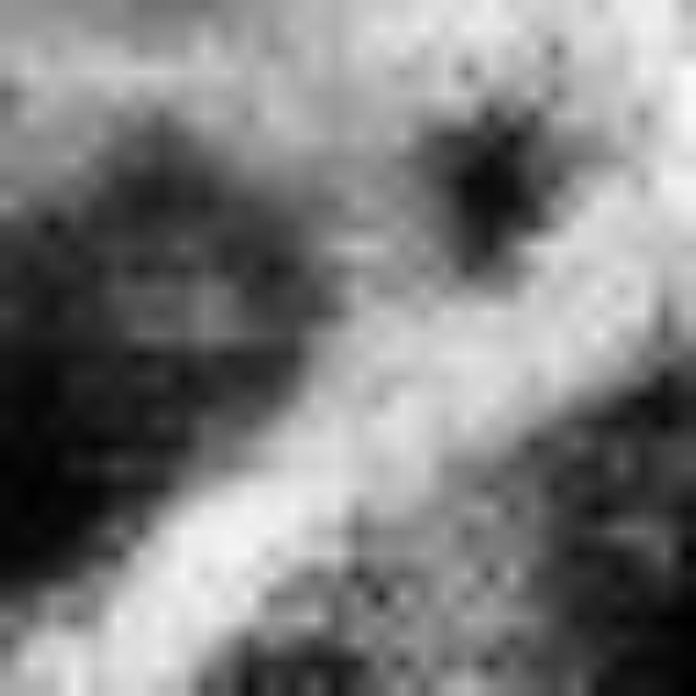
\includegraphics[width=10cm,height=10cm]{sencebgan_reconstruct}};
\pic[shift={(2,0,0)}] at (input_e3-east)
{Box={name=e2test,caption=Stride2,zlabel=5,ylabel=5,fill=\strideColor,height=5,
width=2,depth=5}};
\pic[shift={(2,0,0)}] at (input_e3-east)
{Box={name=e2cvt1,caption=convt1,xlabel={{"128","dummy"}},ylabel=,zlabel=,fill=\eeConvTColor,height=50,width=2,depth=50}};
\pic[shift={(0,0,0)}] at (e2cvt1-east)
{RightBandedBox={name=e2bnlr2,caption=,ylabel=16,zlabel=16,fill=\bnColor,bandfill=\lrColor,height=50,width=2,depth=50}};

% % conv1_1,bn_1, leakyrelu 1
% Stride of convolution
\pic[shift={(2,0,0)}] at (e2bnlr2-east)
{Box={name=e2test,caption=Stride2,zlabel=5,ylabel=5,fill=\strideColor,height=5,
width=4,depth=5}};
\pic[shift={(2,0,0)}] at (e2bnlr2-east)
{Box={name=e2cvt2,caption=convt2,xlabel={{"256","dummy"}},ylabel=,zlabel=,fill=\eeConvTColor,height=40,width=4,depth=40}};
\pic[shift={(0,0,0)}] at (e2cvt2-east)
{RightBandedBox={name=e2bnlr3,caption=,ylabel=8,zlabel=8,fill=\bnColor,bandfill=\lrColor,height=40,width=2,depth=40}};

% % conv1_1,bn_1, leakyrelu 1
% Stride of convolution
\pic[shift={(2,0,0)}] at (e2bnlr3-east)
{Box={name=e2test,caption=Stride2,zlabel=5,ylabel=5,fill=\strideColor,height=5,
width=8,depth=5}};
\pic[shift={(2,0,0)}] at (e2bnlr3-east)
{Box={name=e2cvt3,caption=convt3,xlabel={{"512","dummy"}},ylabel=,zlabel=,fill=\eeConvTColor,height=30,width=8,depth=30}};
\pic[shift={(0,0,0)}] at (e2cvt3-east)
{RightBandedBox={name=e2bnlr4,caption=,ylabel=4,zlabel=4,fill=\bnColor,bandfill=\lrColor,height=30,width=2,depth=30}};
% Final convolution
\pic[shift={(2,0,0)}] at (e2bnlr4-east)
{Box={name=e2cvt3,caption=latent representation,xlabel={{"1","dummy"}},ylabel=32,zlabel=32,fill=\eeConvTColor,height=10,width=16,depth=10}};
% %%%%%%%%%%%%%%%%%%%%%%%%%%%%%%%%%%%%%%%%%%%%%%%%%%%%%%%%%%%%%%%%%%%%%%%%%%%%%%%%%%%%%%%%
% %% Draw Arrow Connections
% %%%%%%%%%%%%%%%%%%%%%%%%%%%%%%%%%%%%%%%%%%%%%%%%%%%%%%%%%%%%%%%%%%%%%%%%%%%%%%%%%%%%%%%%
\draw [connection]  (input_ae-east)        -- node {\midarrow} (cvt1-west); 
\draw [connection](bnlr2-east)        -- node {\midarrow} (cvt2-west); 
\draw [connection]  (bnlr3-east)        -- node{\midarrow} (cvt3-west);

\draw [connection] (img_input-east) -- node{\midarrow} (ecvt1-west);
\draw [connection](ebnlr2-east)        -- node {\midarrow} (ecvt2-west); 
\draw [connection]  (ebnlr3-east)        -- node{\midarrow} (ecvt3-west);

\draw [connection] (input_e3-east) --node{\midarrow} (e2cvt1-west);
\draw [connection](e2bnlr2-east)        -- node {\midarrow} (e2cvt2-west); 
\draw [connection]  (e2bnlr3-east)        -- node{\midarrow} (e2cvt3-west);

\draw [connection] (cvt2-east) -- node{\midarrow} (cv1-west);
\draw [connection] (bnlr_d1-east) -- node{\midarrow} (cv2-west);
\draw [connection] (bnlr_d2-east) -- node{\midarrow} (cv3-west);
\draw [connection] (bnlr_d3-east) -- node{\midarrow} (output-west);

\draw [connection]  (gbnlr1-east)        -- node {\midarrow} (gcvt1-west); 
\draw [connection](gbnlr2-east)        -- node {\midarrow} (gcvt2-west); 
\draw [connection]  (gbnlr3-east)        -- node{\midarrow} (gcvt3-west);

\path (ecvt3-east) -- (input_ae-south|-ecvt3-west) coordinate[pos=0.6] (test);
\path (input_ae-northeast) -- (ecvt3-west|-input_ae-southwest) coordinate[pos=1.4] (ae_bottom);
\path (input_ae-north) -- (input_ae-southwest) coordinate[pos=1.7 ] (test2);
\path (gfc1-north) -- (gfc1-south) coordinate[pos=10.0] (fc-bottom);
\draw [copyconnection] (ecvt3-east) --node{\copymidarrow}(test) --node{\copymidarrow}(ae_bottom) --node{\copymidarrow}(fc-bottom)
--node{\copymidarrow}(gfc1-south);
 
\draw [copyconnection] (img_gen-east) --node[text width=4cm,midway,above]{\textbf{x, G(E(x)) \\ x, G(z)}}
(input_ae-west);

\path (input_ae-north) -- (input_ae-south) coordinate[pos=1.75] (cvt_bottom);
\path (img_gen-north) -- (img_gen-south) coordinate[pos=1.5] (gen_bottom);
\path (input_e3-east) -- (input_e3-west) coordinate[pos=1.5 ] (third_input);

\draw [copyconnection] (img_gen-south) --node{\midarrow}(gen_bottom) --node{\midarrow}(cvt_bottom)
--node{\midarrow}(third_input) --node{\midarrow}(input_e3-west);


\draw [connection]  (-\arrowlength,\up,0) 
node[anchor=south west,scale=2.5]{$z \sim p_{z}$}   
-- node {\midarrow} (0,\up,0);  
%%%%%%%%%%%%%%%%%%%%%%%%%%%%%%%%%%%%%%%%%%%%%%%%%%%%%%%%%%%%%%%%%%%%%%%%%%%%%%%%%%%%%%%%
\end{tikzpicture}
\end{document}